\documentclass{article}
\usepackage[utf8]{inputenc}
\usepackage{graphicx}
\usepackage{amsmath}
\usepackage{amssymb}
\usepackage{algpseudocode}
\usepackage{caption}
\usepackage{xcolor}
\usepackage{float}
\graphicspath{ {./images/} }

\DeclareMathOperator*{\argmax}{arg\,max}
\DeclareMathOperator*{\argmin}{arg\,min}
\DeclareMathOperator{\sech}{sech}
\DeclareMathOperator{\csch}{csch}
\DeclareMathOperator{\arcsec}{arcsec}
\DeclareMathOperator{\arccot}{arcCot}
\DeclareMathOperator{\arccsc}{arcCsc}
\DeclareMathOperator{\arccosh}{arcCosh}
\DeclareMathOperator{\arcsinh}{arcsinh}
\DeclareMathOperator{\arctanh}{arctanh}
\DeclareMathOperator{\arcsech}{arcsech}
\DeclareMathOperator{\arccsch}{arcCsch}
\DeclareMathOperator{\arccoth}{arcCoth} 

\title{\textbf{Homework Assignment II\\Group 42}}
\author{
  91605: Fátima Agostinho Napoleão
  \and
  92447: David Azevedo Escobar de Lima
  \and
  92479: Ielga Katiana Anacleto de Oliveira
}

\date{\textbf{Wednesday, February 2nd, 2022}}

\begin{document}

\maketitle

\section{}

\subsection{}
\textbf{Consider a convolutional neural network (CNN) that takes as input images of size $28 \times 28 \times 3$ and has the following layers:
\begin{itemize}
    \item One convolutional layer with 8 kernels of shape $5 \times 5 \times 3$ with stride of 1, and a padding of zero (i.e., no padding).
    \item A max-pooling layer with kernel size $4 \times 4$ and stride of 2 (both horizontally and vertically).
    \item A linear output layer with 10 outputs followed by a softmax transformation.
\end{itemize}
How many parameters are there in total in this network?}
\begin{itemize}
    \item Image of size = $28 \times 28 \times 3$
    \item Convolutional layer:
        \begin{itemize}
            \item Each Kernel is a matrix of shape 5 x 5
            \item Each kernel has three channels
            \item There are 8 kernels/filters
        \end{itemize}
    \item The total amount of parameters for the convolutinal layer is :
        \begin{itemize}
            \item Number of parameters = number of filters x (( kernel width x kernel height x number of channels) + bias) = 8 x (( 5 x 5 x 3 ) + 1 ))=608
        \end{itemize}
    \item Output Layer:
    \begin{itemize}
        \item As the output is fully connected layer, there are 3 filters 
        \item Number of parameters = numbers of filters x ((input width x input height x number of channels) + bias)
    = 10 x (( 28 x 28 x 3) + 1)
    = 23530
    \end{itemize}
    \item The pooling layer has a fixed operation, so there are no learnable parameters.
    \item The network will have a total of 608 + 23530 = 24138 parameters
        
\end{itemize}
\subsection{}
\textbf{Suppose that we replace the convolutional and max-pooling layers above by a feedforward, fully connected layer with hidden size 100 and output size 10 (followed by the softmax transformation). How many parameters are there in total? Compare to the previous answer and comment.}
\begin{itemize}
    \item Input image of size : $28 \times 28 \times 3$
    \item Fully Connected layer with hidden size 100 and output size 10
    \item A linear output layer with 10 outputs
    \item Fully connected layer parameters:
        \begin{itemize}
            \item Number of parameters = number of units x ((input with x input height x number of channels ) + bias )
            = 100 x ((28 x 28 x 3) + 1) = 235 300
        \end{itemize}
    \item As saw in the previous question there are 23530 parameters for the output layer
    \item Summing all trainable parameters results for each layer, we get the total number of 235300 + 23530 = 258830  parameters within  the entire network
    \item In comparison with others layers a fully connected layer has the highest number of parameters, because all inputs units have a separate weigh to each output unit that's why we have a higher number in this network compared to what we had before.
\end{itemize}




\subsection{}
\textbf{Let $X \in \mathbb{R}^{L \times n}$ be an input matrix for a sequence of length $L$, where $n$ is the embedding size. We are going to look at the self-attention for this sequence. Assume two self-attention heads have projection matrices $W^{(h)}_Q$, $W^{(h)}_K$, $W^{(h)}_V \in \mathbb{R}^{n \times d}$ for $h \in \{1, 2\}$, with $d \leq n$}.

\subsubsection{}
\textbf{Show that the self-attention probabilities for each head can be written as the rows of a matrix of the form
\begin{align}
    \begin{split}
        P^{(h)} = \text{Softmax}(XA^{(h)}X^{\top})
    \end{split}
\end{align}
where $A^{(h)} \in \mathbb{R}^{n \times n}$ has rank $\leq d$ (in the above expression, Softmax is applied row-wise). Provide an expression for the matrix $A^{(h)}$.
}
\begin{itemize}
    \item Given the input $X \in \mathbb{R}^{L \times n}$ for a sequence L, and the self projections matrices $W^{(h)}_Q$,$W^{(h)}_K$,$W^{(h)}_V \in \mathbb{R}^{n \times d}$, $h \in \mathbb{}{{1,2}}$ and $d\leqslant n$
    \item We create the three distance representations:
    \begin{itemize}
        \item Query Vectors : $Q^{(h)} = X W^{(h)}_Q$
         \item Key Vectors : $K^{(h)} = X W^{(h)}_K$
          \item Value Vectors : $V^{(h)} = X W^{(h)}_V$
    \end{itemize}
    \item $P^{(h)} =$ \textbf{Softmax}$(Q^{(h)}(K^{(h)})^{T})$
    \item $P^{(h)} =$ \textbf{Softmax}$(XW^{(h)}_Q(XW^{(h)}_K)^{T}) = $ \textbf{Softmax} $(XW^{(h)}_Q W^{(h)}_K^{T} X^{T})$ 
    \item The $A^{h}$ is given by:
    \begin{itemize}
        \item $A^{h} = W^{(h)}_Q W^{(h)}_K^{T} $
    \end{itemize}
\end{itemize}

\subsubsection{}
\textbf{Show that, if $W^{(2)}_Q = W^{(1)}_Q B$ and $W^{(2)}_K = W^{(1)}_K B^{-\top}$, where $B \in \mathbb{R}^{d \times d}$ is any invertible matrix, then the self-attention probabilities are exactly the same for the two attention heads.}

\begin{itemize}
    \item $h \in {1,2} $
    \item Self-attetion probabilities for first head : h = 1
\begin{itemize}
    \item $P^{(1)} = $ \textbf{Softmax} $  (XA^{(1)}X^{T})$
    \item $A^{(1)} = W^{(1)}_Q W^{(1)}_K^{T}$
\end{itemize}
\item Self-attetion probabilities for the second head : h = 2
\item $P^{(2)} = $ \textbf{Softmax}$(XA^{(2)}X^{T}) = $ \textbf{Softmax}$(XW^{(2)}_Q W^{(2)}_K^{T} X^{T})$
\item $W^{(2)}_Q = W^{(1)}_QB $ and $W^{(2)}_K = W^{(1)}_KB^{-T}$
\item $P^{(2)} = $\textbf{Softmax}$(XW^{(1)}_Q B (W^{(1)}_KB^{-T})^{T}X^{T} =$ \textbf{Softmax}$(XW^{(1)}_Q B(B^{-T})^{T} W^{(1)}_K^{T}X^{T})$
\item Invertible matrix theorems: $B^{-T} = (B^{-1})^{T}$ and $[(B^{-1})^{T}]^{T} = B^{-1}$
\item $P^{(2)} =$ \textbf{Softmax}$(XW^{(1)}_QBB^{-1}W^{(1)}_K^{T}X^{T})$
\item B is invertible \implies $BB^{-1} = I$
\item $P^{(2)}= \textbf{Softmax} $( XW^{(1)}_QIW^{(1)}_K^{T}X^{T} ) \\ = $ \textbf{Softmax}$(XW^{(1)}_QW^{(1)}_K^{T}X^{T})=P^{(1)}$
    
\end{itemize}



\section{}

\textbf{Image classification with CNNs. In this exercise, you will implement a convolutional neural network to perform classification using the Fashion-MNIST dataset. Examples of images in this dataset are shown in Figure 1.}

\begin{figure}[H]
    \centering
    \includegraphics[width=300pt]{images/fig1.png}
    \caption{Examples of images from the Fashion-MNIST dataset.}
\end{figure}

\textbf{As previously done in Homework 1, you will need to download the Fashion-MNIST dataset. You can do this by running the following command in the homework directory:
\begin{align*}
    \begin{tt}
        python \text{ } download\_fashion\_mnist.py
    \end{tt}
\end{align*}
Python skeleton code is provided (\begin{tt}hw2-q2.py\end{tt}). You will now try out convolutional networks. For this exercise, we recommend you use a deep learning framework with automatic differentiation (suggested: \begin{tt}Pytorch\end{tt}).}

\subsection{}
\textbf{What kind of equivariances do convolutional layers exhibit and why are they useful in CNNs for image classification?}\\\\
\begin{itemize}
    \item Locality: because features are translational invariant, small kernels can be used to convolve over the input.
    \item Spatial: this allows for detecting features/objects independently of their position in the input.
\end{itemize}
Because of these two properties, CNNs easily exploit images' data structures. They are capable of learning them independently of their dimensions and use relatively few parameters.

\subsection{}
\textbf{Implement a simple convolutional network with the following structure:
\begin{itemize}
    \item A first block comprising (order as provided):
    \begin{itemize}
        \item A convolution layer with $16$ output channels, a kernel of size $3 \times 3$, stride of $1$, and padding chosen to preserve the original image size.
        \item A rectified linear unit activation function.
        \item A max pooling with kernel size $2 \times 2$ and stride of $2$.
    \end{itemize}
    \item A second block comprising (order as provided):
    \begin{itemize}
        \item A convolution layer with $32$ output channels, a kernel of size $3 \times 3$, stride of $1$, and padding of zero.
        \item A rectified linear unit activation function.
        \item A max pooling with kernel size $2 \times 2$ and stride of $2$.
    \end{itemize}
    \item An affine transformation with $600$ output features (to determine the number of input features use the number of channels, width and height of the output of the second block. (Hint: The $\textbf{number of input features } = \textbf{ number of output channels } \times \textbf{ output width } \times \textbf{ output height}$).
    \item A rectified linear unit activation function.
    \item A dropout layer with a dropout probability of your choice.
    \item An affine transformation with $120$ output features.
    \item A rectified linear unit activation function.
    \item An affine transformation with the number of classes followed by an output LogSoftmax layer.
\end{itemize}
Hint: use the functions \begin{tt}nn.Sequential\end{tt}, \begin{tt}nn.Conv2d\end{tt} and \begin{tt}nn.MaxPool2d\end{tt}.\\\\
Train your model for $15$ epochs using \begin{tt}SGD\end{tt} and tune the learning rate on your validation data, using the following values: $0.001$, $0.01$, $0.1$. For the best configuration, report it and plot two things: the training loss and the validation accuracy, both as a function of the epoch number.
}\\\\
Best configuration: learning rate = 0.01.

\begin{center}
    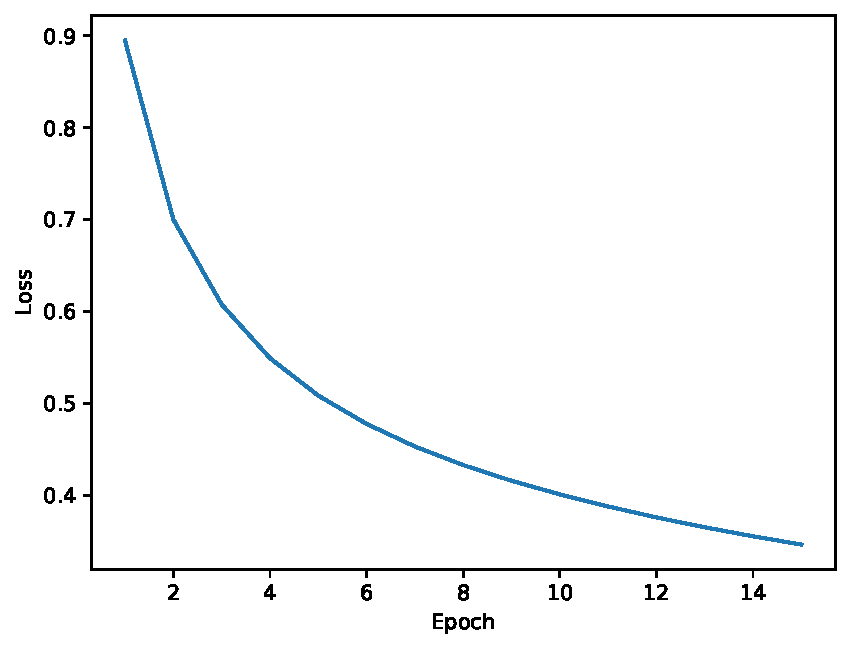
\includegraphics[width=250pt]{images/CNN_0.01/CNN-training-loss-0.01-0.3-0-sgd.pdf}
\end{center}

\begin{center}
    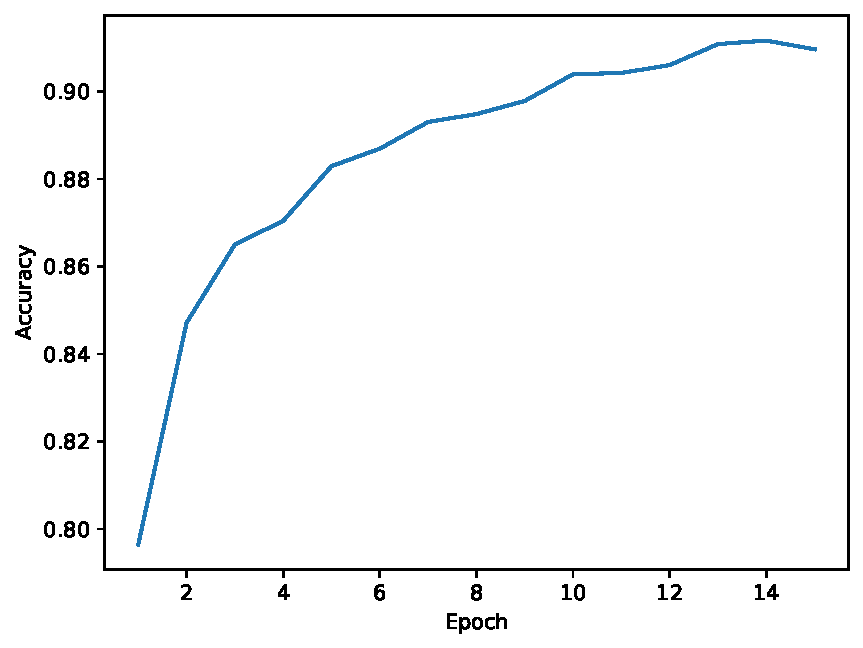
\includegraphics[width=250pt]{images/CNN_0.01/CNN-validation-accuracy-0.01-0.3-0-sgd.pdf}
\end{center}

\subsection{}
\textbf{Plot the filters in the first and second convolutional layers. In general, what kind of features are usually captured by CNNs in bottom vs top layers? (Note: for this exercise, the image resolution may be too low to notice interesting patterns in the filters.)\\\\
NOTE: the skeleton code is designed to output the kernels of the first and second convolutions that you can use to answer the next question. Use the options \begin{tt}-conv\_1\_name\end{tt} and \begin{tt}-conv\_2\_name\end{tt} to save the kernels after finishing the training of the CNN. If you are using \begin{tt}nn.Sequential\end{tt} to define each block as:\\\\
\begin{tt}self.convblock1 = nn.Sequential($\cdots$)\end{tt}\\
\begin{tt}self.convblock2 = nn.Sequential($\cdots$)\end{tt}\\\\
use \begin{tt}-convlayer1 convblock1[0] -convlayer2 convblock2[0]\end{tt}.\\\\
If not using \begin{tt}nn.Sequential\end{tt} and the layers are defined as:\\\\
\begin{tt}self.convlayer1 = nn.Conv2d($\cdots$)\end{tt}\\
$\cdots$\\
\begin{tt}self.convlayer2 = nn.Conv2d($\cdots$)\end{tt}\\\\
use \begin{tt}-convlayer1 convlayer1 -convlayer2 convlayer2\end{tt}.
}\\\\
Layer 1:
\begin{center}
    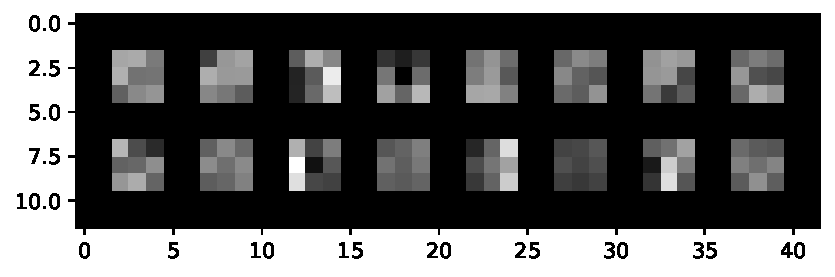
\includegraphics[width=250pt]{images/CNN_Filters/CNN-conv_layer_1_filters-0.01-0.3-0-sgd.pdf}
\end{center}
Layer 2:
\begin{center}
    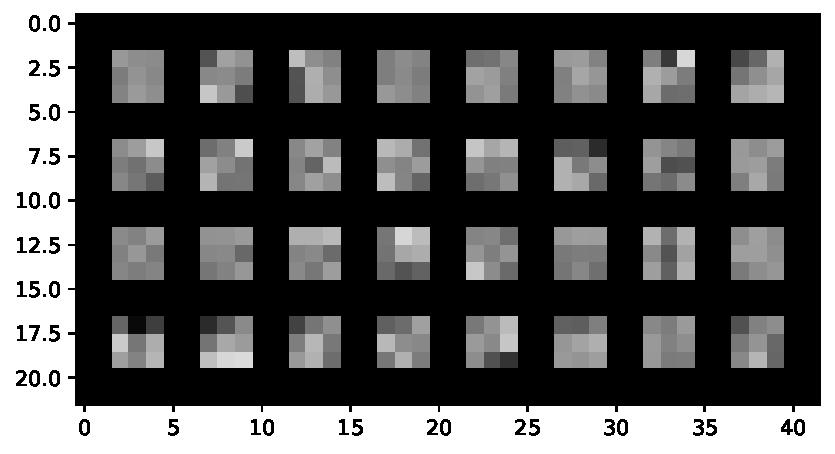
\includegraphics[width=250pt]{images/CNN_Filters/CNN-conv_layer_2_filters-0.01-0.3-0-sgd.pdf}
\end{center}
In general, lower layers capture lower-level representations, such as edges, corners and simple shapes, while higher layers capture higher-level representations, such as specific objects.

\section{}
\textbf{Image Captioning. Image captioning is the problem of automatically describing an image with a short text description. This task is usually addressed with an encoder-decoder model. Typically, the encoder is a CNN model that processes and summarises the input image into relevant feature representations. The representations are then passed to a language decoder, commonly an LSTM model, which generates the respective caption word-by-word given the previous words and the image encoder representations.}

\subsection{}
\textbf{You are going to implement an image captioning model for this task concerning aerial images, thus actually addressing remote sensing image captioning. The input and output should respectively be an image (i.e., remote sensing image) and the corresponding text description. The evaluation metric is BLEU-4 (which calculates precision between n-gram occurrences in the generated and reference captions).}

\subsubsection*{(a)}
\textbf{Unzip the provided \begin{tt}images.zip\end{tt} file and put the images at the \begin{tt}data/raw\_
dataset/images\end{tt} folder.\\\\
Run the file \begin{tt}script\_features.py\end{tt} (\begin{tt}python src/script\_features.py\end{tt}), that extracts the images' features using a pretrained \begin{tt}ResNet-18\end{tt} convolutional neural network encoder model.\\\\
Then, implement a vanilla image captioning model using an encoder-decoder architecture with an auto-regressive LSTM as the decoder. Specifically, in the skeleton code, you will need to implement the method \begin{tt}forward()\end{tt} of the \begin{tt}decoder.py\end{tt} (inside the folder models) and then run (\begin{tt}python3 src/train.py)\end{tt}. \\\\
Plot the training loss and the validation BLEU-4. Also, report the final BLEU-4 score in the test set.\\\\
Hint: At each time-step, the LSTM decoder \begin{tt}self.decode\_step\end{tt} receives as input the embedding of the current word (\begin{tt}self.embedding\end{tt}), then the LSTM hidden state is processed through a dropout operation (\begin{tt}self.dropout\end{tt}), followed by an affine transformation (\begin{tt}self.fc\end{tt}) to produce the scores of the words of the vocabulary.}

\begin{center}
    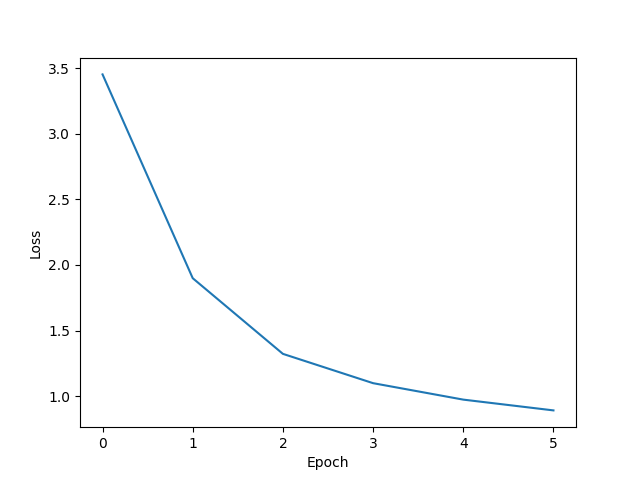
\includegraphics[width=250pt]{images/training_loss_enc_dec.png}
\end{center}

\begin{center}
    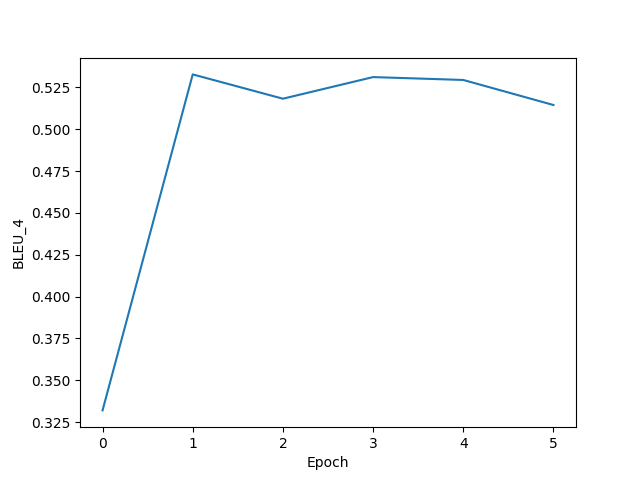
\includegraphics[width=250pt]{images/validation_bleu4_enc_dec.png}
\end{center}

Final BLEU-4 score on test set: 0.52706.

\subsubsection*{(b)}
\textbf{Add an attention mechanism to the decoder (additive attention), which
weights the contribution of the different image regions, according to relevance for the current prediction.\\\\
Specifically, in the skeleton code, you will need to implement the \begin{tt}forward()\end{tt} methods of the \begin{tt}decoder\_with\_attention.py\end{tt}, i.e., the forward methods of the \begin{tt}DecoderWithAttention\end{tt} class and the \begin{tt}Attention\end{tt} class.\\\\
Plot the training loss and the validation BLEU-4. Also, report the final BLEU-4 score in the test set.\\\\
Hint: Now, the input of the LSTM decoder (\begin{tt}self.decode\_step\end{tt}) is the embedding of the current word (\begin{tt}self.embedding\end{tt}) concatenated with the attention vector.\\\\
You can run the code with the command
\begin{align*}
    \begin{tt}
        python \textbf{ } src/train.py \text{ } -use\_attention
    \end{tt}
\end{align*}}

\begin{center}
    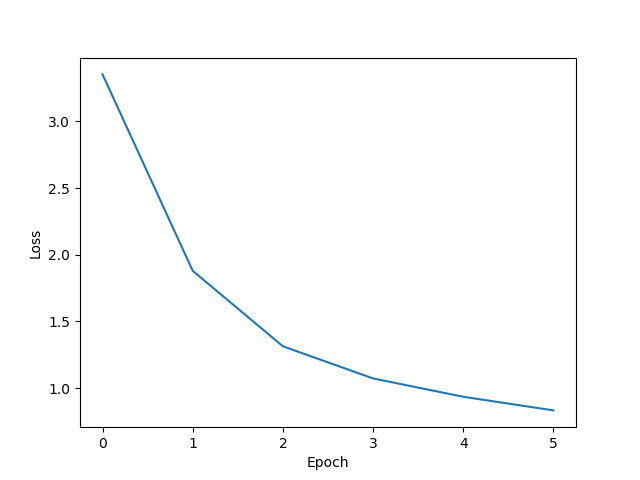
\includegraphics[width=250pt]{images/training_loss_enc_dec_w_attention.png}
\end{center}

\begin{center}
    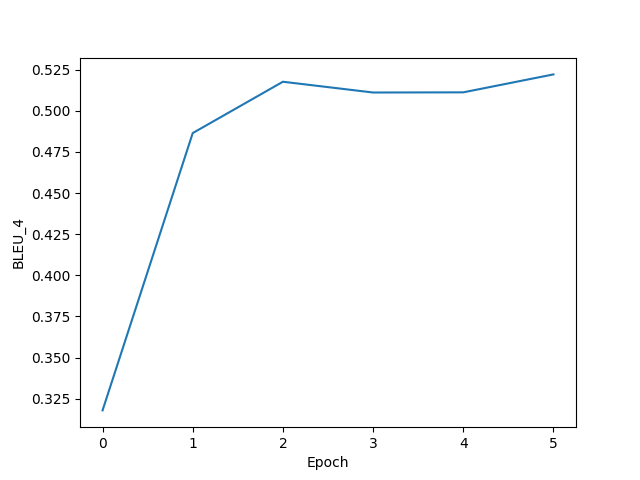
\includegraphics[width=250pt]{images/validation_bleu4_enc_dec_w_attention.png}
\end{center}
Final BLEU-4 score on test set: 0.52922.

\subsubsection*{(c)}
\textbf{For the previous model (encoder-decoder with neural attention), report the generated captions for the images "\begin{tt}219.tif\end{tt}", "\begin{tt}540.tif\end{tt}", "\begin{tt}357.tif\end{tt}". For each of those images, place the image next to the corresponding caption. \\\\
Hint: Use the file inside the results folder:
\begin{align*}
    \begin{tt}
        caps\_generated\_enc\_dec\_w\_attention.json.
    \end{tt}
\end{align*}}

\begin{figure}[H]
    \centering
    \includegraphics[width=230pt]{images/219.png}
    \captionsetup{labelformat=empty}
    \caption{\textbf{219:} "a residential area with many houses arranged neatly and some roads go through this area"}
\end{figure}

\begin{figure}[H]
    \centering
    \includegraphics[width=230pt]{images/540.png}
    \captionsetup{labelformat=empty}
    \caption{\textbf{540:} "an industrial area with many white buildings and some roads go through this area"}
\end{figure}

\begin{figure}[H]
    \centering
    \includegraphics[width=230pt]{images/357.png}
    \captionsetup{labelformat=empty}
    \caption{\textbf{357:} "a residential area with many houses arranged neatly and some roads go through this area"}
\end{figure}

\end{document}
